\documentclass[12pt]{article}
\usepackage[utf8]{inputenc}
\usepackage{mathtools}
\usepackage{amsmath}
\usepackage{derivative}
\usepackage{amsthm}
\usepackage{amssymb}
\usepackage{listings}
\usepackage{hyperref}
\usepackage{tikz}
\usepackage{float}
\usepackage{float}
\usepackage{algorithm}
\usepackage{algpseudocode}
\usepackage{graphicx}
\graphicspath{{./figures/}}
\usetikzlibrary{arrows,decorations.pathmorphing,backgrounds,positioning,fit,matrix}
\usepackage[symbols,nogroupskip,record]{glossaries-extra}
\usepackage[
backend=biber,
style=alphabetic,
sorting=ynt
]{biblatex}
\addbibresource{references.bib}

\newfloat{algorithm}{H}{lop} % flaot the alg environment

\glsxtrnewsymbol[description={position},location={[see sec.~\ref{ch1}].}]{x}{\ensuremath{x}}
\glsxtrnewsymbol[description={velocity},location={[see sec.~\ref{ch1}].}]{v}{\ensuremath{v}}
\glsxtrnewsymbol[description={acceleration},location={[see sec.~\ref{ch1}].}]{a}{\ensuremath{a}}
\glsxtrnewsymbol[description={time},location={[see sec.~\ref{ch1}].}]{t}{\ensuremath{t}}
\glsxtrnewsymbol[description={gap},location={[see sec.~\ref{ch1}].}]{s}{\ensuremath{s}}
\glsxtrnewsymbol[description={desired speed (typically $33$ m/s)},
location = {[see ch.~\ref{ch3.1}]}]{v0}{\ensuremath{v_0}}
\glsxtrnewsymbol[description={desired speed (typically $3$ m)},
location = {[see sec.~\ref{ch3.1}]}]{s_0}{\ensuremath{s_0}}
\glsxtrnewsymbol[description={desired speed (typically $1.4$ s)},
location = {[see sec.~\ref{ch3.1}]}]{T}{\ensuremath{T}}
\glsxtrnewsymbol[description={adaptation time (typically $5$ s$^{-1}$)}]{tau}{\ensuremath{\tau}}
\glsxtrnewsymbol[description={speed difference sensitivity (typically $0.6$ s$^{-1}$)}]{ga}{\ensuremath{\gamma}}

\title{Investigating Car Following Model}
\author{Kaeshav Danesh and Kevin Phan}
\date{\today}

\begin{document}
    \maketitle

    \begin{abstract}
        Traffic flow dynamics is generally split into either macroscopic models or microscopic models. For this paper, we will focus on car following models which is a type of microscopic model. We first introduce the assumptions and the mathematical description car following model and the numerical scheme used to compute them. Then, we give the full velocity difference model. Finally, we examine different scenarios such as bottlenecks and lane changes and analyze the behavior of cars. 
    \end{abstract}

    \newpage

    \tableofcontents

    \newpage

    \section{Introduction}
    How does a bottleneck affect a series of vehicles? What impact does changing a road from multiple lanes to one lane have a series of cars? To answer these questions, our paper will describe a basic microscopic car following model from traffic flow theory, implement these scenarios, and analyze them. 

    Traffic flow models can be categorized as microscopic or macroscopic models [\cite{hisTraffic}]. Microscopic models describe vehicles on the individual level by treating them as entire unit. Meanwhile, macroscopic models treat vehicles as a continuum. Further classifications can be done through the model equations such as partial differential equations, discrete equations, discrete or continuous variables, and deterministic or stochastic process. Some applications of traffic flow models include simulating traffic, optimizing traffic lights, and calculating carbon emissions from traffic. 

    Our paper will focus only on the microscopic model called the Full Velocity Difference model. Using this model, we will explore scenarios including bottlenecks, phantom traffic, and lane changes. From this, we will analyze state variables including position, velocity, and acceleration, and other metrics such as density and flow rate. 
    % Some questions to answer:
    % \begin{itemize}
    %     \item Why are traffic models important? Applications?
    %     \item At what scale does our model operate at? Macroscopic and %     microscopic?  
    %     \item What assumptions are we making? 
    % \end{itemize}

    \section{General Model}
    \subsection{Mathematical Formulation}\label{ch1}
        We follow the mathematical formulation of car following model in \S 10.2 of \cite{traffic}. Suppose that there are $n$ vehicles in the simulation using the car following model. We index the $1$st vehicle by $1$, the $2$nd car by $2$, the $\alpha$th car by $\alpha$, and so on. The state variables of vehicle $\alpha$ are position $x_\alpha$, velocity $v_\alpha$, and acceleration $a_\alpha$. Furthermore, we are also assuming that the vehicles in the model has a length $l$. The position $x_\alpha$ of car $\alpha$ is defined as the front bumper of the car. Another useful variable to define is gap. We define the gap of car $\alpha$ by the difference in distance between the back bumper of car $\alpha - 1$ and the front bumper of car $\alpha$. Mathematically, the gap $s_\alpha$ is defined as 
        \begin{equation} 
          s_\alpha = x_{\alpha - 1} - l_{\alpha -1}  - x_{\alpha}
        \end{equation}
        where $x_{\alpha - 1}$ is the position of car $\alpha - 1$, $l_{\alpha - 1}$ is the length of car $\alpha - 1$, and $x_\alpha$ is the position of car $\alpha$. We note that the gap is not defined for a vehicle with no vehicles in front of it. 
        \begin{figure}[H]
            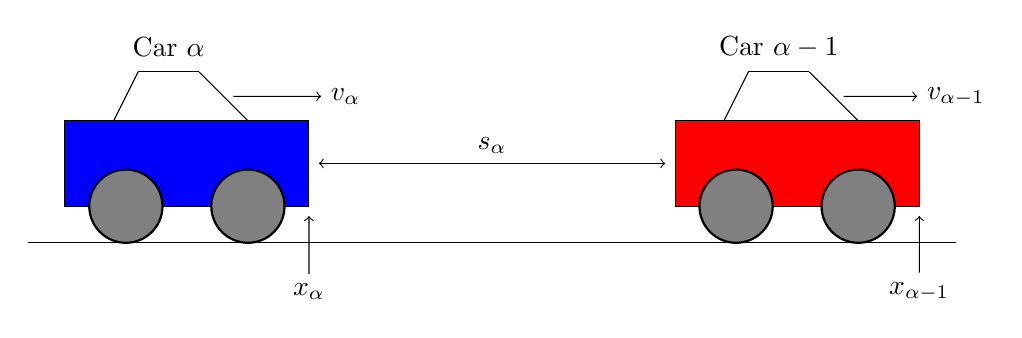
\begin{tikzpicture}[scale=1.55]
                \draw (-0.3,-0.3) -- (7.3,-0.3);
                \draw [fill = blue] (0,0) rectangle (2,0.7);
                \draw [fill=gray, thick] (0.5,0) circle [radius=0.3];
                \draw [fill=gray, thick] (1.5,0) circle [radius=0.3];
                \draw (1.5,0.7) -- (1.1,1.1);
                \draw (1.1,1.1) -- (0.6,1.1);
                \draw (0.6,1.1) -- (0.4,0.7);
                \node (car_a-1) at (0.85,1.3) {Car $\alpha$};
                \node (vel) at (2.3,0.9) {$v_{\alpha}$};
                \node (vel_start) at (1.3,0.9) {};
                \draw[->] (vel_start) -> (vel);
                \begin{scope}[shift={(5,0)}]
                    \draw [fill = red] (0,0) rectangle (2,0.7);
                    \draw [fill=gray, thick] (0.5,0) circle [radius=0.3];
                    \draw [fill=gray, thick] (1.5,0) circle [radius=0.3];
                    \draw (1.5,0.7) -- (1.1,1.1);
                    \draw (1.1,1.1) -- (0.6,1.1);
                    \draw (0.6,1.1) -- (0.4,0.7);
                    \node (car_a-1) at (0.85,1.3) {Car $\alpha - 1$};
                    \node (vel) at (2.3,0.9) {$v_{\alpha - 1}$};
                    \node (vel_start) at (1.3,0.9) {};
                    \draw[->] (vel_start) -> (vel);
                  \end{scope}
                \node (x) at (2,0.35) {};
                \node (y) at (5,0.35) {};
                \node (x_pos) at (2,0) {};
                \node (x_sym) at (2,-0.7) {$x_{\alpha }$};
                \node (x_pos1) at (7,0) {};
                \node (x_sym1) at (7,-0.7) {$x_{\alpha - 1}$};
                \draw[<->] (x) -- node[above] {$s_{\alpha}$} (y);
                \draw[<-] (x_pos) -- (x_sym);
                \draw[<-] (x_pos1) -- (x_sym1);
                \end{tikzpicture} 
            \centering
            \caption{Defining index, position, velocity, and gap of a car.}
        \end{figure}  
        For simpler notation, we will now refer to the vehicle in front of vehicle $\alpha$ by the leader vehicle $l$. For a single lane, car $l$ is vehicle $\alpha - 1$. However, it is not necessarily true that vehicle $l$ is vehicle $\alpha - 1$ for multiple lanes. 

        Taking the time derivatives of $x_\alpha (t)$ and $v_\alpha (t)$ lead to the general coupled differential equation describing velocity and acceleration respectively: 
        \begin{align} 
          \odv{x_\alpha(t)}{t} &= v_\alpha (t), \\
          \odv{v_\alpha (t)}{t} &= a_{\rm mic} (s_\alpha, v_\alpha, v_l).
        \end{align}
        Each car following model has a specific acceleration function: $a_{\rm mic}\footnote{We use $a_{\rm mic}$ for the acceleration function and $a$ to describe the state variable acceleration.}$. For the simulation, we will use the Full Velocity Difference Model (FVDM) which is described in section (\ref{ch3.1}).
    \subsection{Numerical Scheme}\label{num_sch}
    The standard way of numerically solving a system of coupled differential equations would be to use a fourth order Runge Kutta method.
    However, higher order methods all assume higher orders of smoothness in the differential equation and its solution [\cite{numerics}].
    Our model is only smooth to first order because suddenly changes in acceleration is common, for example, during lane changes. 
    So, using a high order method could be worse than a simple first order method.

    Among first order methods, our options are either the forward or backwards (implicit) Euler methods. The main difference between these methods is that the backwards Euler method involves solving an implicit equation and is generally more stable.

    We are using the forward Euler method because we expect our solution to be stable and solving an implicit equation every timestep would add extra complexity to our implementation.

    Implementing the forwards Euler method scheme for a car following model gives us two coupled differential equations for each of our states:
    \begin{align}
        v_\alpha(t+\Delta t) &= v_\alpha(t) +a_{\rm mic}(s_\alpha(t), v_\alpha (t), v_l (t))\Delta t, \label{num_eq1}\\
        x_\alpha(t + \Delta t) &= x_\alpha(t) + \frac{v_\alpha (t) + v_\alpha (t+\Delta t)}{2}\Delta t \label{num_eq2},
    \end{align}
    where $\Delta t$ is the time step and $a_{\rm mic}$ is the acceleration function defined by the car following model used. This acceleration function is described in section(\ref{ch3.1}).

    When solving the equations above numerically, we must also consider the interactions between cars. The velocity equation uses $v_l(t)$, the velocity of the leading car at time $t$. So, when calculating the state of a car at each timestep, it would be easier to start from the backmost car and work up. This allows us to use the most recent velocity value from the leading car.     

    \section{Car Following Model}
    \subsection{Full Velocity Difference Model}\label{ch3.1}
    We followed the details of the Full Velocity Difference Model in \S 10.6 and \S 10.7 of [\cite{traffic}]. The Full Velocity Difference Model (FVDM) is given by the acceleration function: 
    \begin{equation}\label{a_mic}
      a_{\rm mic}(s_\alpha,v_\alpha,v_l) = \frac{v_{\rm opt} (s) - v_\alpha}{\tau} - \gamma \Delta v 
    \end{equation}
    where $v_{\rm opt}$ is the optimal velocity function, $\tau$ is the speed adaptation time, $\gamma$ is the speed difference sensitivity, and $\Delta v = v_\alpha - v_l$ is the difference between in velocities of the car $\alpha$ and the leader car.
    
    A simple choice for $v_{\rm opt}$ is 
    \begin{equation} 
      v_{\rm opt} (s) = \max \left( 0, \min \left( v_0, \frac{s-s_0}{T} \right) \right)
    \end{equation}
    where $v_0$ is the desired speed, $s_0$ is the minimum distance gap, and $T$ is the time gap. 

    Typical parameters for highway traffic for the FVDM is given in the table below. 
    \begin{figure}[H]
      \begin{center}
        \begin{tabular}{l c c } 
        Parameter & Value \\
        \hline
        $v_0$, desired speed & $33.\bar{3}$ m/s \\
        $s_0$, minimum distance gap & $3$ m \\
        $T$, time gap & $1.4$ s \\
        $\tau$, speed adaptation time & $5$ s \\
        $\gamma$, speed difference sensitivity & $0.6$ s$^{-1}$ \\
        \end{tabular}
        \end{center}
        \caption{Typical parameters for highway traffic for the FVDM.}
        \label{fig:parameters}
    \end{figure}
    
    We now examine how different parameters of the optimal velocity function affect the graph. 
    \begin{figure}[H]
        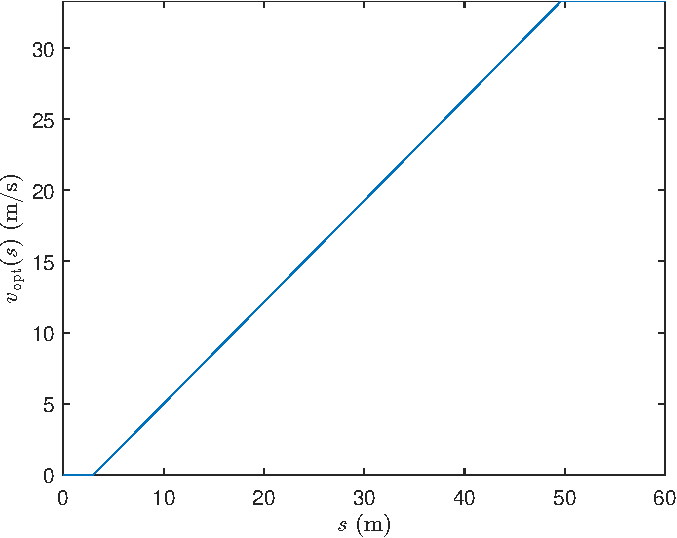
\includegraphics[width=11cm]{vopt_versus_s.pdf}
        \centering
    \end{figure}
    Since we are taking the minimum of $v_0$ and $(s-s_0)/T$, $v_{\rm opt}$ attain a maximum of $v_0$. This means that the optimal velocity of a vehicle is the desired speed $v_0$. Furthermore, $v_{\rm opt}$ is $0$ on the interval $0 \leq s \leq s_0$ which means that a vehicle will not move if the vehicle's gap is $s_0$ or less. This prevents car crashes from occurring for most cases. Lastly, the time gap $T$ determine the slope of the line. Higher values of $T$ means that the car's optimal velocity will be reached for higher value of $s$.
    
    Analyzing equation (\ref{a_mic}), $v_{\rm opt} (s) - v_\alpha$ is positive if $v_{\rm opt} (s) > v_\alpha$. The car has not reached its optimal velocity and so, acceleration is positive. Similarly, if  $v_{\rm opt} (s) < v_\alpha$, $v_{\rm opt} (s) - v_\alpha$ is negative and so, the car is decelerating to reach its optimal velocity. If $v_{\rm opt} (s) = v_\alpha$, then $a_{\rm mic} = 0$. The speed adaptation time $\tau$ determine how fast the car accelerate or decelerate and thus, affect the time it takes for the car to reach its optimal velocity. The term $-\gamma \Delta v$ is positive if $v_\alpha < v_l$ and negative if $v_\alpha > v_l$. This leads to more acceleration if the car is trying to catch to the leader car and less acceleration if the car is trying to slow down due to the leader car's slower velocity. 
  
    \subsection{Implementation}\label{sec:implementation}
    We first initialize initial conditions for the state variables of the vehicles. We store the vehicles in an array and iterate through them. As described in section (\ref{num_sch}), we iterate through the vehicles starting with the last vehicle with respect to position and go through in ascending order. We update the state variables of the cars using equations (\ref{num_eq1}), (\ref{num_eq2}), and (\ref{a_mic}). We repeat this process for the number of iterations required. 
    \begin{algorithm}
      \caption{Simplified algorithm for FDVM}\label{alg:car-following}
      \begin{algorithmic}
      \Require Initial state variables for each car at $t=0$. 
      \Require carArr, an array of cars.
      \For{$i = 1:$numsteps}{}
      \For{$j =$ length(carArr):$-1$:$1$}{}
        \State State variables of $j$th car $\gets$ Update $j$th car by a timestep.
        \EndFor
      \EndFor
      \end{algorithmic}
      \end{algorithm}
    We still have not addressed the situation with the first car when updating its state variables. The equation (\ref{a_mic}) need values for the car's gap $s_\alpha$ we are updating and the velocity of the leader car $v_l$. However, the first car does not have a leader car. To resolve this, we impose a destination for the cars. We use this value in the calculation of gap $s_\alpha$ by computing $x_\alpha - x_{\rm destination}$. For the situation of the velocity of the leader car, it might be reasonable to set it to set $v_l = 0$. However, if $v_l=0$, then the term $-\gamma \Delta v$ blow up. In other words, this car is too wary of crashing. To resolve this problem, it is best to set $v_l = v_\alpha$ which ensure that the term $-\gamma \Delta v$ is $0$. However, we note that this will cause a small problem in our simulation. We will address this in section (\ref{sec:homogeneous_pitfal}). 
    
    We use the same parameters in Figure (\ref{fig:parameters}). Furthermore, we choose the width of the cars to be $5$ meters.
    \section{Examining Different Scenarios}
    \subsection{Homogeneous Traffic}
    TODO: Give basic graphs so that we can compare to in the next sections and add any pitfalls with the model (unrealistic acceleration), Look at the pitfalls (since gap is used, stuff from far away can affect it and unrealistic acceleration which can be included in section 4.1 maybe?)
    \subsubsection{Data}
    In this section, we will present multiple graphs from our simulation. We present graphs of position, velocity, acceleration, and gap. These graphs will be used to compare the graphs we get from later sections. 
    
    We will do a simulation with the algorithm described in section (\ref{sec:implementation}). At $t=0$, the initial conditions are $x_\alpha = 
    200-\frac{200}{9}\left(a-1\right)$, $v_\alpha = 0$, and $a_\alpha = 0$ for $1 \leq \alpha \leq 10$. 
      \begin{figure}[H]
          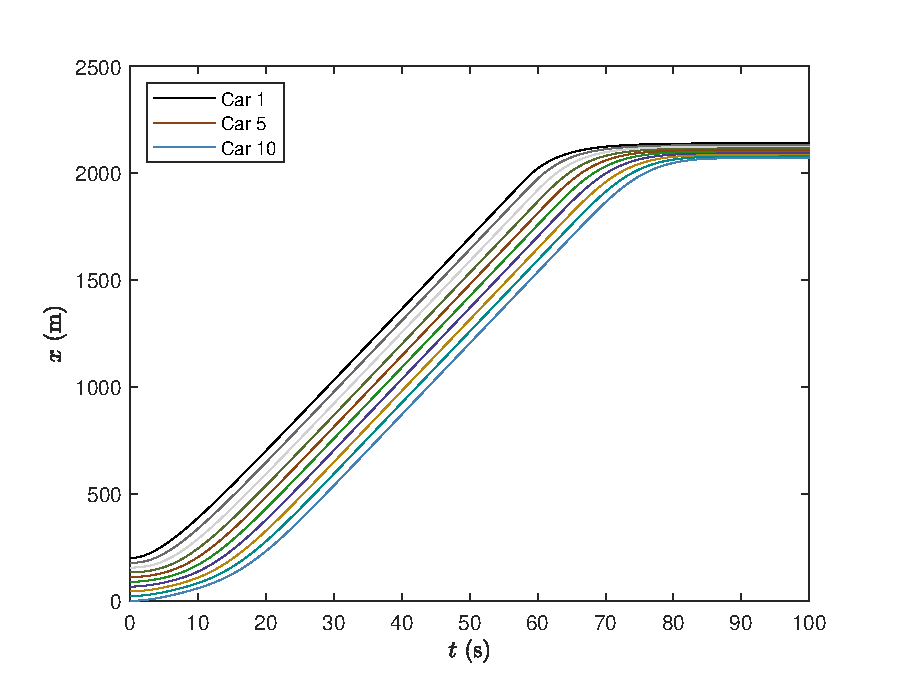
\includegraphics[width=11cm]{HomogeneousTraffic1.eps}
          \centering
          \caption{Position versus time graph.}
      \end{figure}

      \begin{figure}[H]
        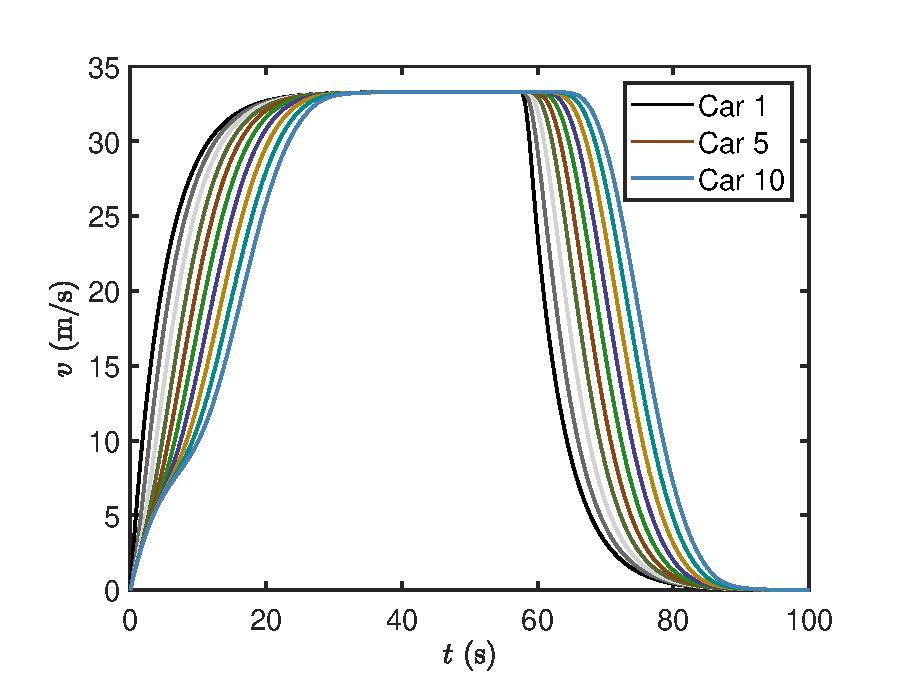
\includegraphics[width=11cm]{HomogeneousTraffic2.eps}
        \centering
        \caption{Velocity versus time graph}
      \end{figure}

      \begin{figure}[H]
      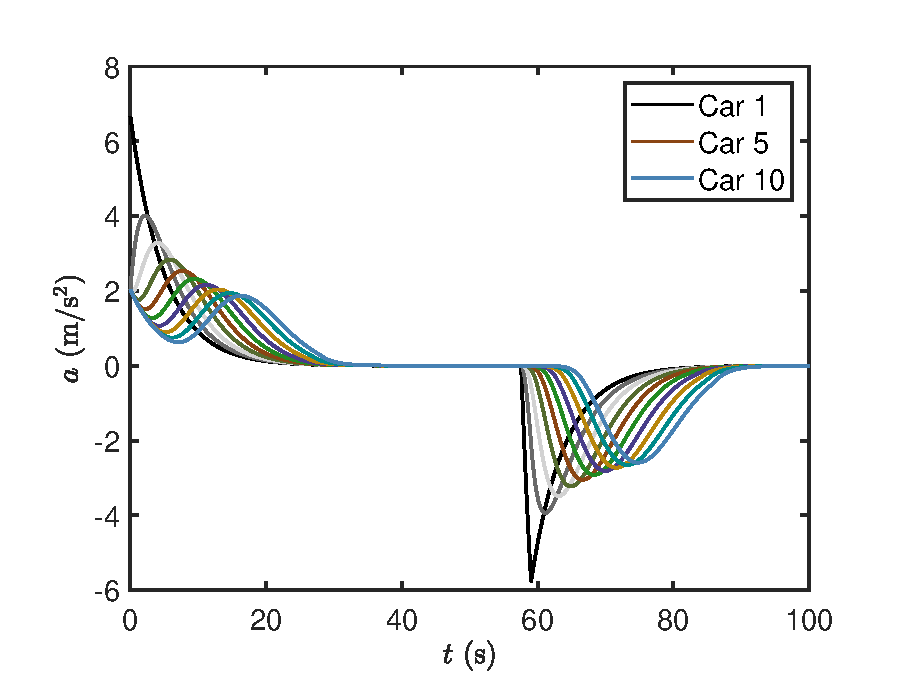
\includegraphics[width=11cm]{HomogeneousTraffic3.eps}
      \centering
      \caption{Acceleration versus time graph}
      \end{figure}

      \begin{figure}[H]
      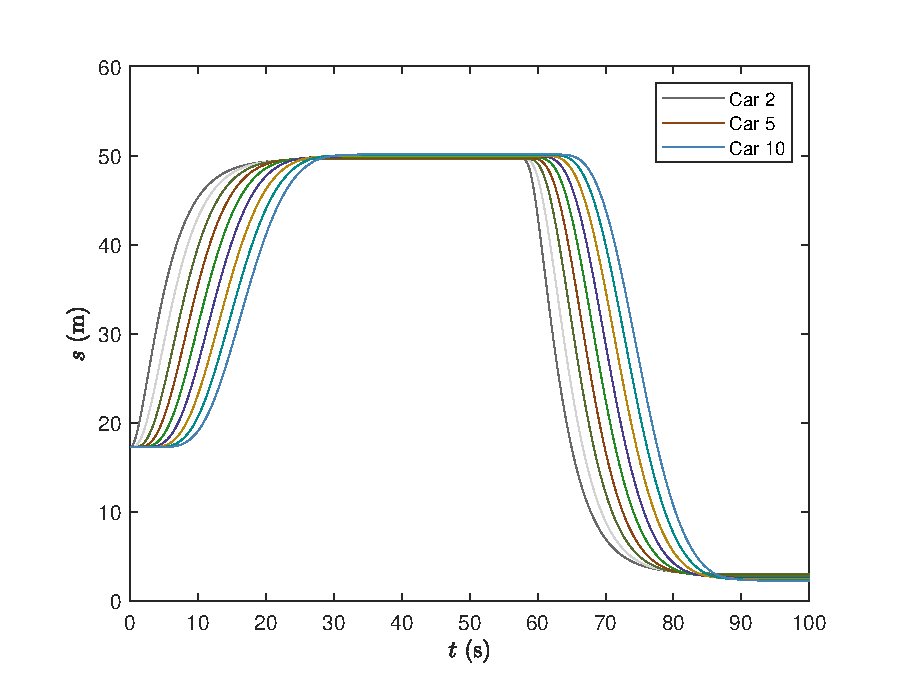
\includegraphics[width=11cm]{HomogeneousTraffic4.eps}
      \centering
      \caption{Gap versus time graph}
      \end{figure}
      
      For the gap versus time graph, we do not plot the gap of car $1$ since the gap is the difference between the car position $x_1$ and $x_{\rm position}$ which is not of interest. 
    \subsubsection{Pitfalls}\label{sec:homogeneous_pitfal}
    There is one pitfall with how we update the first car's acceleration. In section \ref{sec:implementation}, we choose $v_l = v_\alpha$ and $s_\alpha = x_{\rm destination} - x_\alpha$ where $\alpha = 1$. The problem with solution is that it simulate a car that is permanently stuck at $x_{\rm destination}$ but with the same velocity as the first car. When the first car approaches $x_{\rm destination}$, the model predict that it is safe to move past $x_{\rm destination}$ since the simulated car has non-zero velocity and so, it will move out of the way. This does not happen and so, the car move past $x_{\rm destination}$. Due to how $v_{\rm opt}$ is computed, $v_{\rm opt}$ is $0$ once the first car is past $x_{\rm destination}$. In other words, the first car does eventually slow down and stop. It is better to state that $x_{\rm destination}$ is when the first car will begin to slow down and eventually stop after some distance.  
    \subsection{Bottleneck}
    TODO: Add time versus position graph and label the different situations, density graph, analysis, page 11 is a good source of questions to ask for this, a graph of car versus difference in time to get there (use the previous section)
    \subsubsection{Implementation}
    \subsubsection{Data}
    \subsubsection{Analysis}
    \subsection{Lane Changes}
    TODO: Average lane speed (How much faster is one lane with and without lane changes) and bottleneck revisted (make it from 2 lanes to one lane) and how number of lanes affect flow rate. The grass is greener on the other side paradox (in the textbook) 
    \subsubsection{Implementation}

   Lane changes are dealt with on a microscopic level, meaning that for in each timestep for each vehicle, we decided whether or not to change lanes.  In our model, we will only consider changing to adjacent lanes in a single time step (no sideways driving). So, in timestep $t$, vehicle number $\alpha$ has three choices: go left, go right, or stay in the same lane.

      \begin{figure}[H]
        \begin{center}
          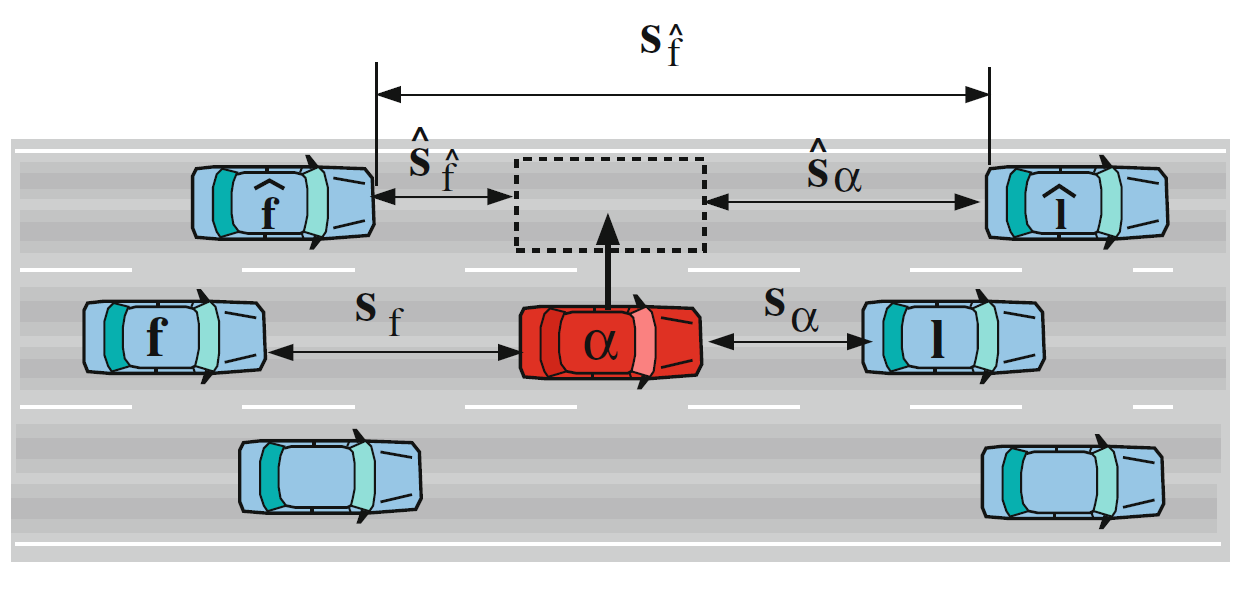
\includegraphics{lane_change_diagram.PNG}
        \end{center}
        \caption{An example of the notation we are using for lane changes. $l$ denotes the leading car and $f$ denotes the following car. A hat refers to quantities after the lane change. From page $242$ in [\cite{traffic}].}
      \end{figure}

      When a vehicle decides to change lanes, it must do two things: check that the lane change is safe and check that there is an incentive to change lanes.

      Checking to see if a lane change is safe is straightforward. All the vehicle must do is ensure that $s_{\alpha}$ is smaller than a predefined safe gap. This minimum gap is dependent on factors like the velocities of the vehicles and the reaction time of the drivers. 
      Considering this, we can define a minimum safe gap as 
      \begin{equation}
        s_{\rm safe} (v_{\hat f}, v_{\alpha}) = v_{\rm opt}^{-1} \left[v_{\hat f} -\tau b_{\rm safe} + \tau \gamma (v_{\hat f} - v_{\hat a}) \right]
      \end{equation}
      where $b_{\rm safe}$ is the limit for a safe deceleration and $\tau$ is the adaptation time. 

      TODO: Explain inverse optimal velocity function.

      To check the incentive, we need to consider the gap in the current lane, the gap in the lane we want to switch to, and the velocities of the leading cars in both lanes. We only want to switch lanes if there is either a large gap in the other lane or if the leading car in the other lane is faster. Therefore, we can define a gap, $s_{\rm adv}$, that encapsulates the benefit of staying in the same lane. 
      
      To prevent erratic lane changes, we also need to define an advantage threshold $\Delta a$ such that the vehicle will only change lanes if potential gain in acceleration is greater than $\Delta a$.  Left lanes are also usually designated as passing lanes, so right lanes are slower by convention. So, we introduce $a_{\rm bias}$ which lets our model prefer the left lane over the right one. 
      
      Combining all of the factors above gives us a measure of the cost of changing lanes:
      \begin{equation}
        s_{\rm adv} = s_{\alpha} + s_e\left[\tau(\Delta a + a_{\rm bias} + \gamma(v_l - v_{\hat l})).\right]
      \end{equation}

      So, a vehicle can only change lanes if $\hat s_{\hat f} > s_{\rm safe}$ and $\hat s_{\alpha} > s_{\rm adv}$. 

      Typical lane changing parameters in a highway are given in the table below. 
      \begin{figure}[H]
        \begin{center}
          \begin{tabular}{l c c } 
          Parameter & Value \\
          \hline
          $b_{\rm safe}$, limit for safe deceleration & $2$ m/s$^2$ \\
          $\Delta a$, changing threshold & $0.1$ m/s$^2$ \\
          $a_{\rm bias}$, keep left directive & $0.3$ m/s$^2$ in right lane, $-0.3$ in left lane \\

          \end{tabular}
          \end{center}
          \caption{Typical parameters for highway traffic for the lane changing algorithm. From page 244 in [\cite{traffic}]}
          \label{fig:parameters}
      \end{figure}

      When adding the lane changing algorithm to our existing code, we must ensure that the order of the cars are tracked during every timestep because $a_{\rm mic}$ and the lane changing algorithm rely. If one car overtakes another, the array of cars will go out of order. We alleviated this by reordering our array of cars at the end of each timestep.  
      \begin{algorithm}
        \caption{Simplified algorithm for FDVM with lane changes}\label{alg:car-following-lane}
        \begin{algorithmic}
        \Require Initial state variables for each car at $t=0$. 
        \Require carArr, an array of cars.
        \For{$i = 1:$numsteps}{}
        \For{$j =$ length(carArr):$-1$:$1$}{}
          \State State variables of $j$th car $\gets$ Update $j$th car by a timestep.
          \State New lane of $j$th car $\gets$ carArr($j$).changeLane()
          \EndFor
          \State sort(carArr)
        \EndFor
        \end{algorithmic}
        \end{algorithm}
    \subsubsection{Pitfall}
    TODO: Talk about how lane change alg. can only change lanes from left to right (no capable of taking a bunch of costs at once and to get an advantage)
    \subsection{Multi-lane Bottleneck}
    An example of a multi-lane bottleneck is construction on the side of a highway. We can examine what happens when two lanes of a three-lane highway are closed for maintenance. 
    \subsubsection{Implementation}
    To implement the closure of two lanes, we placed two virtual vehicles. One was at lane one with a width of 1100 and the front at 2000. The other vehicle was in lane two and had a width of 1000 with the front also at 2000. So, lane three was the lane that was left empty.
    \subsubsection{Data}

    \begin{figure}[H]
      \begin{center}
        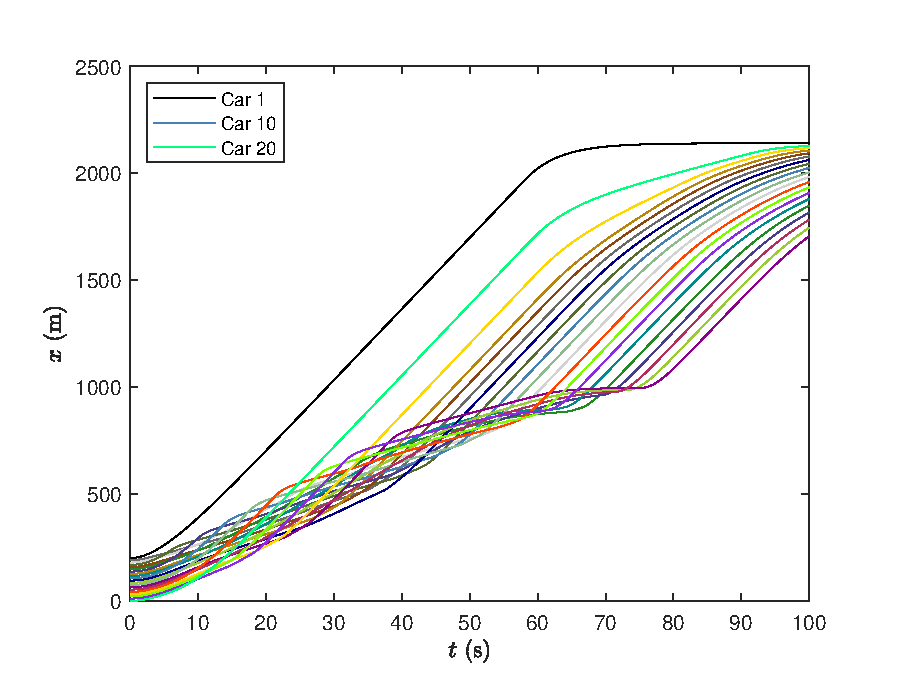
\includegraphics[width=13cm]{mlbn_x.eps}
        \caption{Position versus time graph. Each line represents a single vehicle, and vehicles in all lanes are shown. Car 1 started in lane 3.}
        \label{multi lane x}
      \end{center}
    \end{figure}

    \begin{figure}[H]
      \begin{center}
        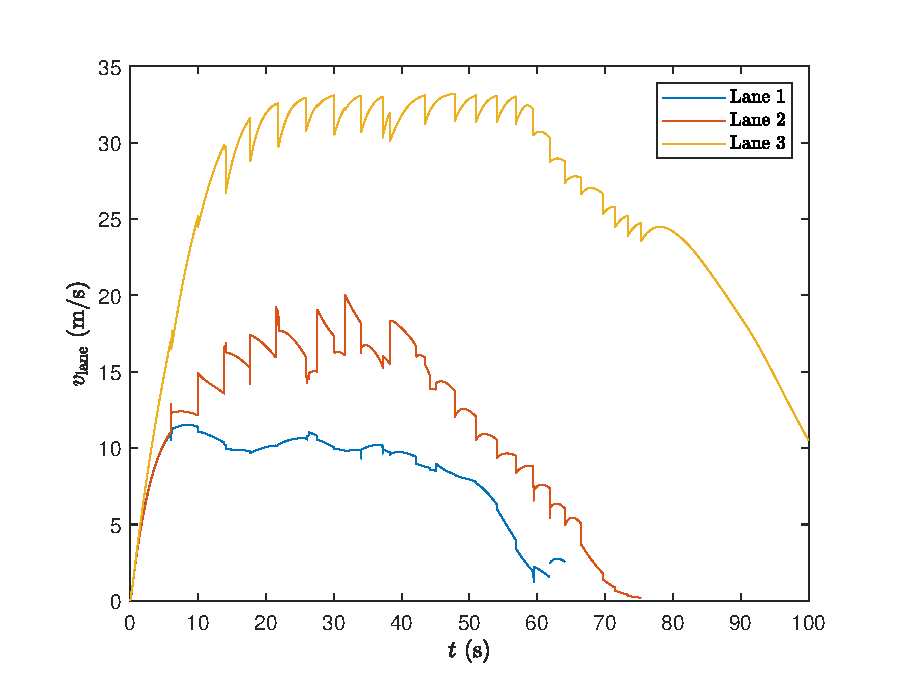
\includegraphics[width=13cm]{mlbn_laneSpeed.eps}
        \caption{Mean speed of vehicles in each lane  }
        \label{mean lane speed}
      \end{center}
    \end{figure}

    \begin{figure}[H]
      \begin{center}
        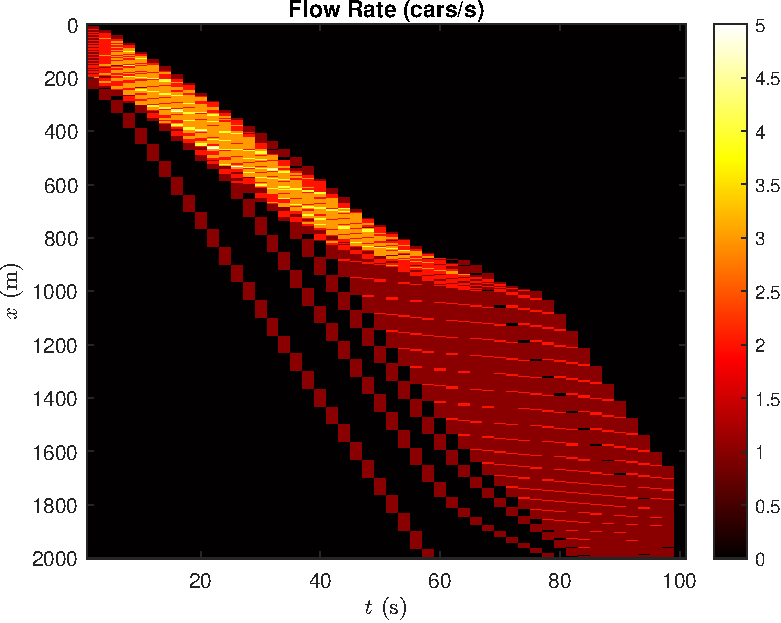
\includegraphics[width=13cm]{mlbn_flow.pdf}
        \caption{Flow rate versus time (s) and position (m)}
      \end{center}
    \end{figure}

    \begin{figure}[H]
      \begin{center}
        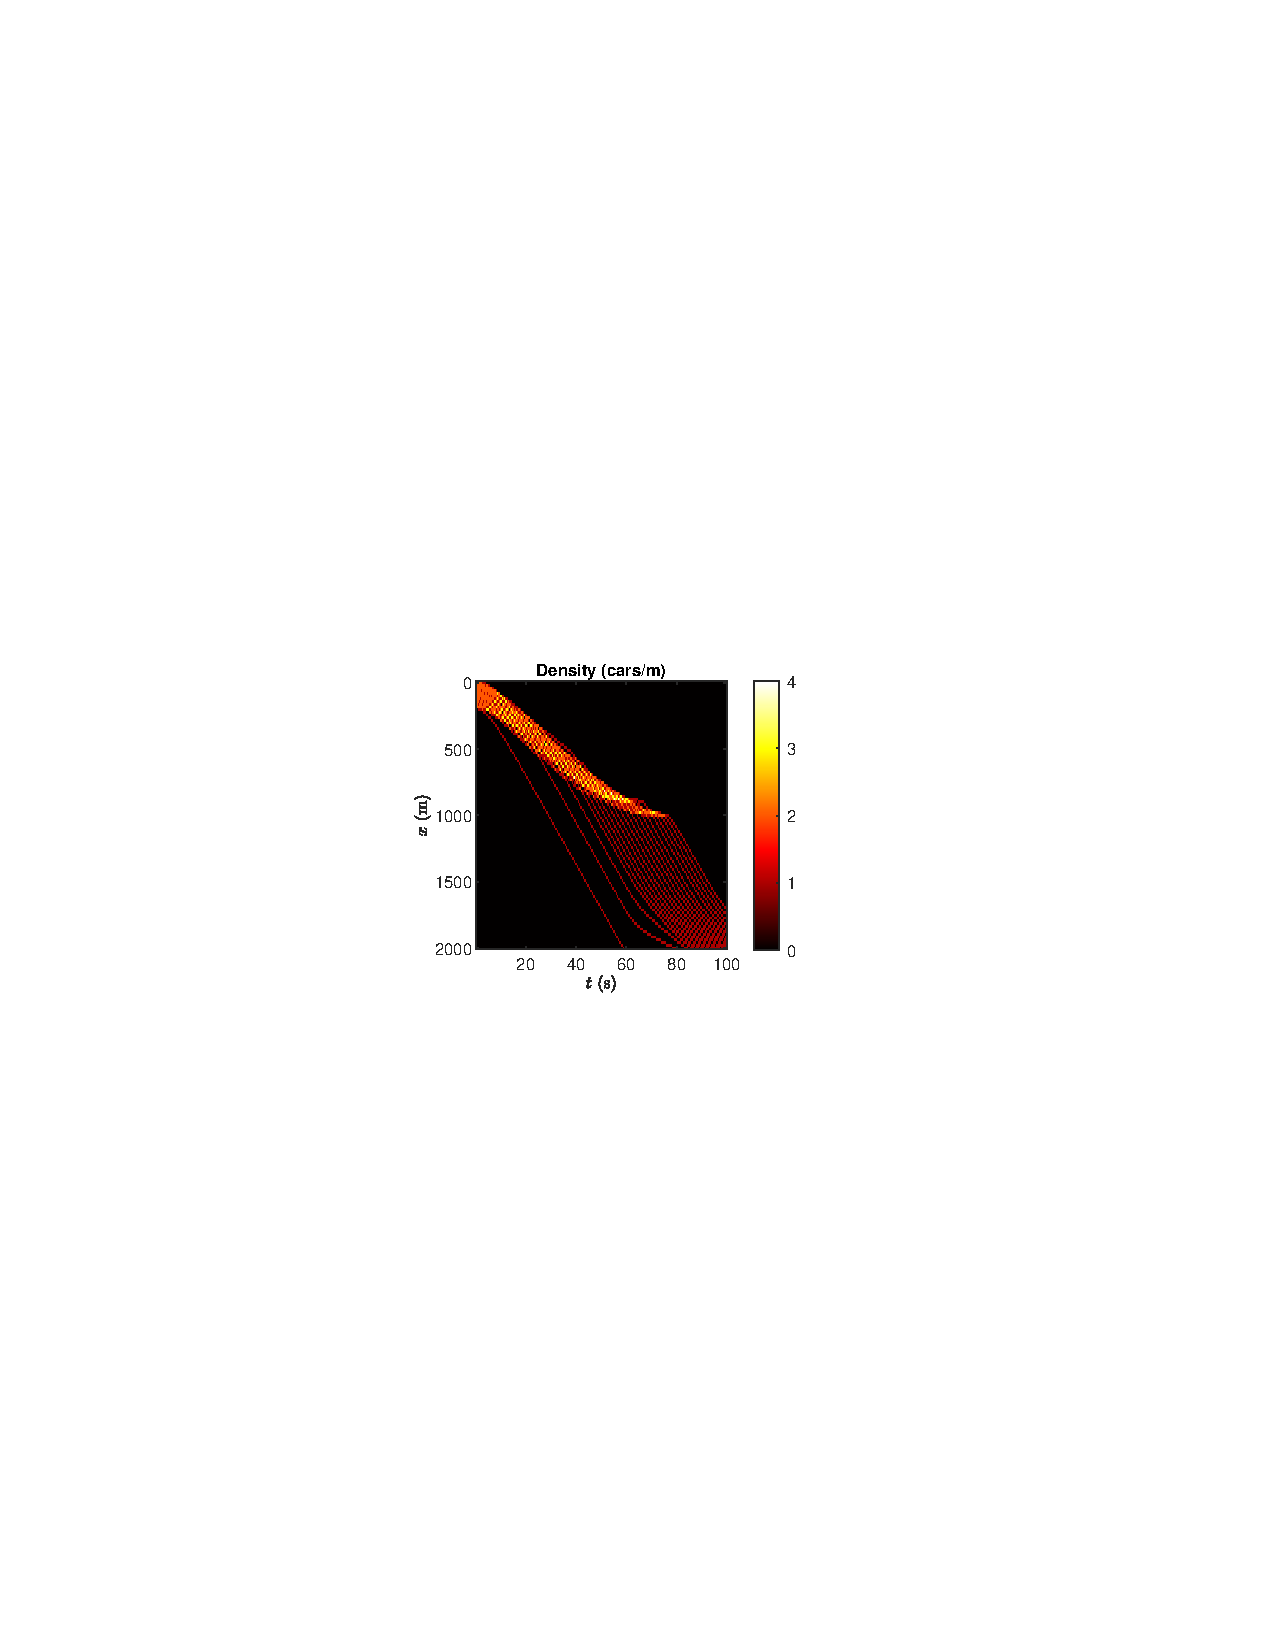
\includegraphics[width=13cm]{mlbn_density.pdf}
        \caption{Density versus time (s) and position (m)}
        \label{num cars per lane}
      \end{center}
    \end{figure}

    TODO: Some way of representing lane data. Perhaps a heatmap with cars in y axis, time in x axis.

    \begin{figure}[H]
      \begin{center}
        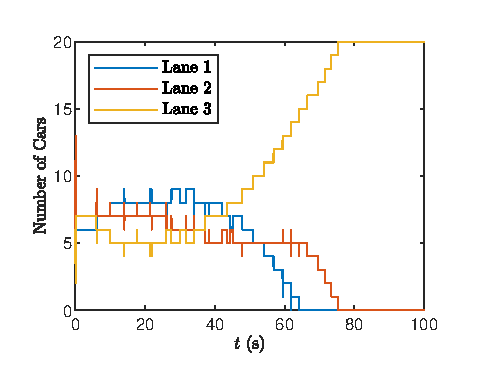
\includegraphics[width=13cm]{mlbn_lanecars.eps}
        \caption{Number of cars per lane}
      \end{center}
    \end{figure}
    \subsubsection{Analysis}

    In figure (\ref{multi lane x}), most of the cars appear to slow down before the roadblock at $x = 900$ except for Car one. This is likely caused by the cars in the front slowing down and changing to the empty lane in anticipation of the roadblock. Since Car one starts of in the empty lane and is the first car, it is able to avoid the traffic caused by lane changes farther back.
   
    From figure (\ref{mean lane speed}), the mean speed of cars in lane three are much higher than those in lanes one and two. There are a lot of sudden dips in $v-{\rm lane}$ for lane three and these dips correspond with sudden peaks in Lane two. This is caused by cars changing lane from two to three, hence cars in lane two speed up because of the larger gaps and cars in lane three decelerate to maintain a larger gap.

    TODO: Interpret figure 11. We can see in Figure 11 that flow rate is much higher before the roadblock and it appears to spread out. In Flow rate graphs, intensity is conserved?

    TODO: Interpret figure 12 or get rid of it.

    Figure (\ref{num cars per lane}) confirms that all cars eventually end up in lane three. There is a sharp decrease of cars in lane one at $t=50$ and a decrease of cars in lane two at $t = 70$. 

    \section{Conclusion}
    \section{Further Remarks}
    \printunsrtglossary[type=symbols,style=long,title={List of Symbols and Constants}]
    \newpage 
    \printbibliography
\end{document}